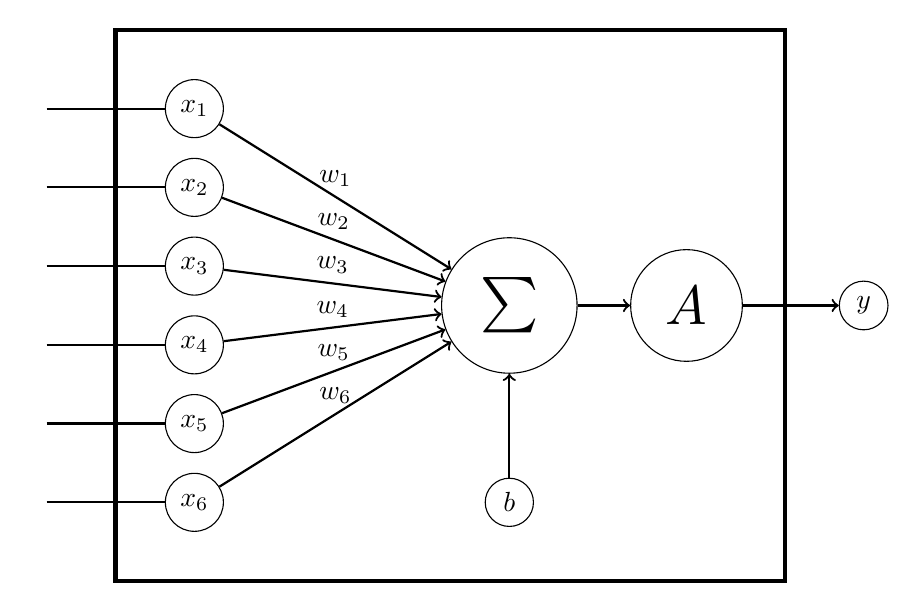
\begin{tikzpicture}
  \node (f1) at (-2, 0) {};

  \node[draw, circle] (X1) at (0, 0){
    $x_{1}$
  };

  \node (f2) at (-2, -1) {};

  \node[draw, circle] (X2) at (0, -1){
    $x_{2}$
  };

  \node (f3) at (-2, -2) {};

  \node[draw, circle] (X3) at (0, -2){
    $x_{3}$
  };

  \node (f4) at (-2, -3) {};

  \node[draw, circle] (X4) at (0, -3){
    $x_{4}$
  };

  \node (f5) at (-2, -4) {};

  \node[draw, circle] (X5) at (0, -4){
    $x_{5}$
  };

  \node (f6) at (-2, -5) {};

  \node[draw, circle] (X6) at (0, -5){
    $x_{6}$
  };

  \node[draw, circle] (bias) at (4, -5){
    $b$
  };

  \node[draw, circle] (sum) at (4, -2.5){
    \scalebox{2}{
      $\sum$
    }
  };

  \node[draw, circle] (activation) at (6.25, -2.5){
    \scalebox{2}{
      $A$
    }
  };


  %% \uncover<2->{
  %%   \node[draw, circle] (activation) at (6.25, -2.5){
  %%     \scalebox{2}{
  %%       $A$
  %%     }
  %%   };
  %% }

  \node[draw, circle] (y) at (8.5, -2.5){
    $y$
  };

  \draw[thick] (f1) -- (X1);
  \draw[thick] (f2) -- (X2);
  \draw[thick] (f3) -- (X3);
  \draw[thick] (f4) -- (X4);
  \draw[thick] (f5) -- (X5);
  \draw[thick] (f6) -- (X6);

  \draw[thick, ->] (X1) -- node [above]{$w_{1}$} (sum);
  \draw[thick, ->] (X2) -- node [above]{$w_{2}$} (sum);
  \draw[thick, ->] (X3) -- node [above]{$w_{3}$} (sum);
  \draw[thick, ->] (X4) -- node [above]{$w_{4}$} (sum);
  \draw[thick, ->] (X5) -- node [above]{$w_{5}$} (sum);
  \draw[thick, ->] (X6) -- node [above]{$w_{6}$} (sum);
  \draw[thick, ->] (bias) -- (sum);
  %% \uncover<1>{
  %%   \draw[thick, ->] (sum) -- (y);
  %% }
  %% \uncover<2->{
  %%   \draw[thick, ->] (sum) -- (activation);
  %%   \draw[thick, ->] (activation) -- (y);
  %% }
  \draw[thick, ->] (sum) -- (activation);
  \draw[thick, ->] (activation) -- (y);

  \path [ultra thick, draw] (-1, 1) -- (7.5, 1) rectangle (-1, -6) -- (7.5, -6);
\end{tikzpicture}
